\documentclass{article}

\usepackage[hidelinks]{hyperref}
\usepackage{enumitem}
\usepackage{amsfonts}
\usepackage[framemethod = tikz]{mdframed}

\usepackage{geometry}
\geometry{
	a4paper,
	top=3cm,
	bottom=3cm,
	left=2.5cm,
	right=2.5cm,
	heightrounded,
	bindingoffset=0mm
}

\hypersetup{
	colorlinks=false,
	linkcolor=blue,
	filecolor=magenta,
	urlcolor=cyan,
	linktocpage=false
}

\usepackage{listings}
\usepackage{titlesec}

\newcommand\chaptername{Section}
\titleformat{\section}[display]{\normalfont\huge\bfseries}{\chaptername\ \thesection}{20pt}{\Huge}
\titlespacing*{\section}{0pt}{50pt}{40pt}
\newcommand\sectionbreak{\clearpage}

\title{ 
	
\includegraphics[width=95mm]{img/PolimiLogo.png} \\
	\bigskip
	Design Document (DD)
}

\author{
	Davide Rossetto 894029, Alessandro Tatti 883861
}

\date{
	Delivery date: 2017 Nov 26\\
	\bigskip v0.9
}

\begin{document}
	
\maketitle
\newpage
\tableofcontents
\newpage
	
	
	\section{Introduction}
	

	\subsection{Purpose}
	The structure of the following document is divided into two sections:
	\begin{enumerate}
	\item Design Document (main section)
	\item Integration Test Plan Document (secondary section)
	\end{enumerate}

	\bigskip
	The Design Document (DD) is intended to provide a more detailed functional description of the Travlendar + system – to - be by providing technical details and describing the main architectural components, their interfaces, and their interactions.
	
	The relationships among the different modules are highlighted using UML standards and other useful diagrams that show the structure of the system.
	
	The document has to guide the software development team to implement the project architecture, providing a stable reference and a unique view of all parts of the software, defining their operation.

	\bigskip
	The second part of the document is intended to provide guidelines to adequately carry out the planning of the integration test phase.
	
	The document includes determining which necessary tools, drivers and data structures that will be useful during the test process.

	
	
	\subsection{Scope}
	The system aims to support a personal event management service, providing features for choosing the best path, means of transport, and insertion of the break. The system must also make sure there are no overlap among meetings and among meetings and breaks.

	The system is structured with a four-layer architecture. The purpose of the document is to describe this architecture in detail.

	\bigskip
	The system described is suitable for different types of customers: different actors that interact with the system - to – be by generating a client-server dualism, so the flow of requests and responses.
	
	The architecture must be designed with the intention of being maintainable and extensible, to make future possible changes.
	
	\bigskip
	This document aims to guide the implementation phase so that cohesion and decoupling are increased as much as possible. In order to do this, individual components must not include too many independent functions and reduce interdependence.
	
	This document will follow specific architectural styles and design templates used for future implementation, as well as common design paradigms that combine useful features of this concepts.


	
	\subsection{Definitions, Acronyms, Abbreviations}
	\begin{description}
	\item [ACID:] Atomicity, Consistency, Isolation and Durability. This is the set of properties of database transactions.
	\item [API:] Application Programming Interface.
	\item [DD:] Design Document.
	\item [DBMS:] DataBase Management System.
	\item [E-R diagram:] entity – relationship diagram.
	\item [EJB:] Enterprise JavaBean.
	\item [HTTPS:] HyperText Transfer Protocol over Secure Socket Layer.
	\item [IE:] Internet Explorer. 
	\item [ITPD:] Integration Test Plan Document.
	\item [JAX - RS:] Java API that provides support in creating web services according to the REST pattern.
	\item [JEE:] Java Enterprise Edition.
	\item [JPA:] Java Persistence API.
	\item [JSON:] JavaScript Object Notation
	\item [MVC:] Model-View-Controller.
	\item [NGINX:] Web Server used in the Web Server Implementation.
	\item [RASD:] Requirements Analysis and Specification Document.
	\item [REST:] REpresentational State Transfer. It is a way of providing interoperability between computer systems on the Internet.
	\item [RESTful:] a REST compliant system.
	\item [Swift:] language used for developing iOS apps.
	\item [UIKit:] the framework provides the required infrastructure for your iOS.
	\item [UML:] Unified Modeling Language.
	\item [UX:] User Experience.
	\item [XML:] eXtensible Markup Language
	\end{description}
	
	
	\subsection{Revision history}
	\begin{description}
		\item [v0.1] Construct basic document's structure, add \textit{Overview}.
		\item [v0.2] Add \textit{Purpose}, \textit{Scope}, \textit{Definitions, Acronyms, Abbreviations}, \textit{Reference documents} and \textit{Document structure}.
		\item [v0.3] Add \textit{High level components}, \textit{Appendix} and \textit{Bibliography}.
		\item [v0.4] Add \textit{Component view}.
		\item [v0.5] Add \textit{Deployment view}, \textit{Runtime view}, \textit{Component interfaces}, \textit{Architectural styles and patterns} and \textit{Other design decisions}.
		\item [v0.6] Add \textit{Requirements Traceability} and \textit{UX diagrams}.
		\item [v0.7] Add \textit{Algorithm Design}.
		\item [v0.8] Add \textit{Implementation, Integration and Test Plan}.
		\item [v0.9] Syntactical review.
		\item [v1.0] First delivery.
	\end{description}
	
	
	\subsection{Reference documents}
	This document follows the guidelines provided by ISO/IEC/IEEE 1016:2009 [3] related to system design and software design descriptions for complex software systems.

	\bigskip
	The indications given in this document are based on those given in the previous delivery for the project, the RASD document [1].
	
	\bigskip
	This document is strictly based on the RASD assignment [2] and the test plan example presented during the lessons for the project of Software Engineering II, course held by Elisabetta Di Nitto and Matteo Giovanni Rossi at the Politecnico di Milano, A.Y. 2017/2018.
	
	
	\subsection{Document structure}

	This document consists of six sections:

	\begin{description}
	\item [Section 1:] Introduction. This section provides a general introduction and overview of the Design Document and the covered topics that were not previously taken into account by the RASD [1].
	\item [Section 2:] Architectural Design. This section shows the main system components together with sub-components and their relationship. This section is divided into different parts whose focus is mainly on design choices, interactions, architectural styles and patterns.
	\item [Section 3:] Algorithm Design. This section focuses on the definition of the most relevant algorithms to be implemented by the system – to – be.
	\item [Section 4:] User Interface Design. It provides an overview on how the user interface will look like.
	\item [Section 5:] Requirements Traceability. This section explains how the requirements you have defined in the RASD [1] map to the design elements that you have defined in this document.
	\item [Section 6:] Implementation, Integration and test plan. This section identifies the order in which the developer plan to implement the subcomponents of the system and the order in which he plans to integrate such subcomponents and test the integration.
	\end{description}

	\bigskip
	At the end of the document are an Appendix and a Bibliography, providing additional information about the sections listed above.

	\section{Architectural Design}
	
	\subsection{Overview}

	This section gives a detailed overview of physical and logical infrastructures of the system-to-be and describes the main components and their interactions.

	A top-down approach is adopted for the description of the architectural design of the system:

	\bigskip
	\begin{description}
	\item [High level components:] a description of the high-level components and their interactions.
	\item [Component view:] a detailed vision of the components described in the previous section.
	\item [Deployment view:] a set of guidelines on how to deploy the components on physical tiers.
	\item [Runtime view:] a detailed vision of the dynamic behavior of the software.
	\item [Component interfaces:] a description of the different interfaces.
	\item [Architectural styles and patterns:] a set of Architectural styles, design patterns and paradigms used in the design phase.
	\item [Other design decisions:] a list of all relevant decisions taken during the design process and not mentioned before.
	\end{description}


	\subsection{High level components}

	The high-level components of the system are the following:

	\begin{description}
	\item [Database:] the \textit{Data Layer} of the system; all the data structures and entities concerning data storage. This level does not contain any application logic.
	\item [Application Server:] the layer that contains all the \textit{application logic} and \textit{key algorithms} of the system.
	\item [Web Server:] the Layer that provides all the \textit{web pages} to the \textit{web-based application}. This level does not contain any application logic.
	\item [Mobile Application:] the \textit{Presentation Layer} of the \textit{mobile application}; This level does not contain any application logic.
	\item [Web Browser:] the \textit{Presentation Layer} of the \textit{web-based application}; It just renders the pages obtained from the \textit{Web server} and executes its scripts.
	\end{description}

	\begin{figure}[!ht]
	\centering
	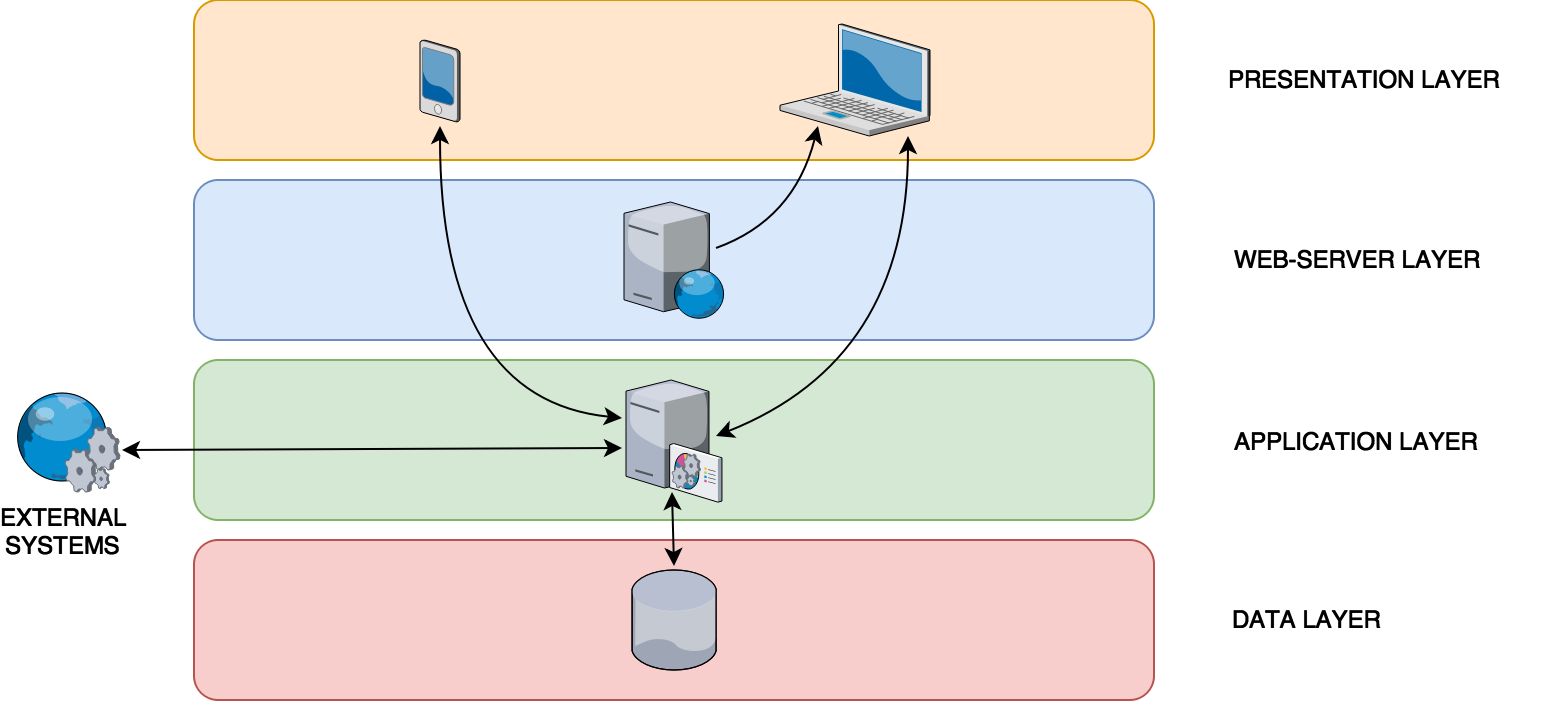
\includegraphics[width=0.95\textwidth]{img/diagrams/layers.png}
	\caption{Layer structure of the system.}
	\end{figure}

	\bigskip
	\begin{figure}[!ht]
	\centering
	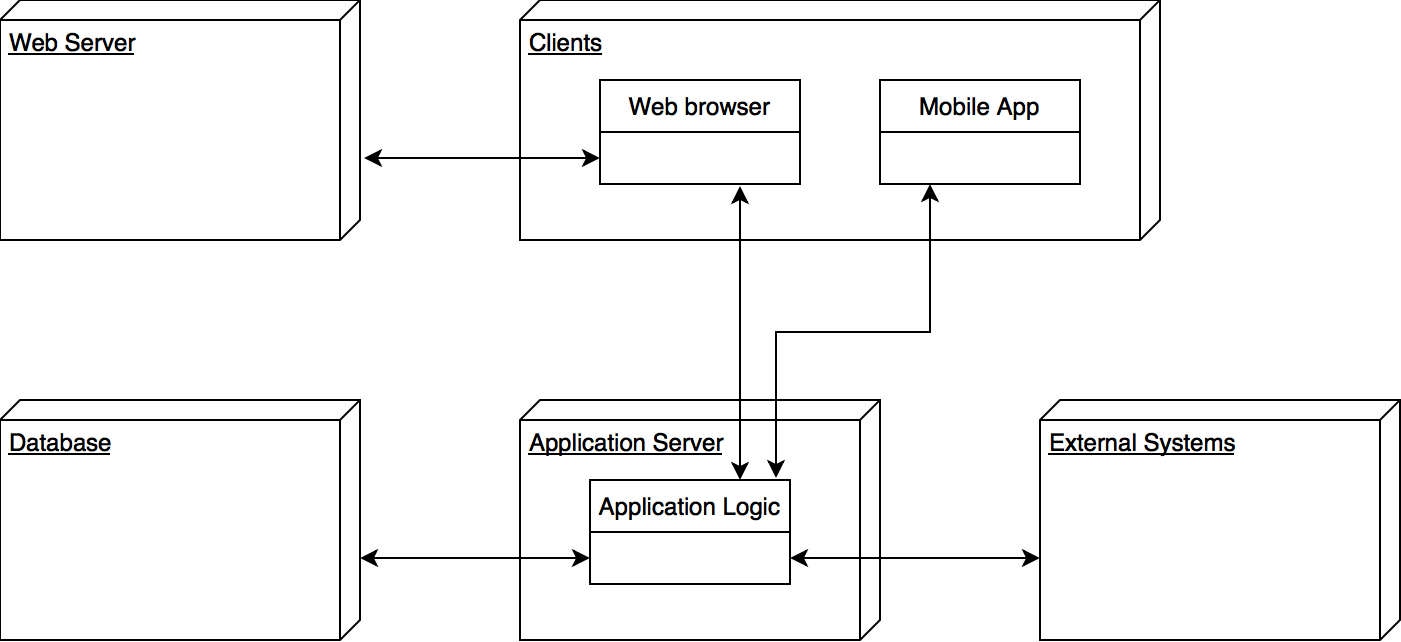
\includegraphics[width=0.75\textwidth]{img/diagrams/hlc.png}
	\caption{High-level components of the system.}
	\end{figure}

	\newpage

	\subsection{Component view}

	This section shows in a more detailed way the components introduced in the overview, their role and their interactions.

	\subsubsection{Database}
	The database layer must include a DBMS component in order to manage the insertion, modification, deletion, and registration of data transactions within the storage memory.
	
	The DBMS must guarantee the correct functioning of simultaneous transactions and ACID properties; the DBMS must be relational because the requirements of the application in terms of data storage do not require a more complex structure than the one provided by the relational data structure.
	
	The data layer must be accessible only through Application Server via a dedicated interface. The Application Server must provide a persistence unit to handle the dynamic behavior of all persistent application data.
	
	The database must be optimized during the implementation phase to ensure security by granting access to data according to the applicant's privilege level. Sensible data, for example passwords and personal information, must be encrypted correctly before being stored. Users must be granted access only on the provision of correct and valid credentials.

	\begin{figure}[!ht]
	\centering
	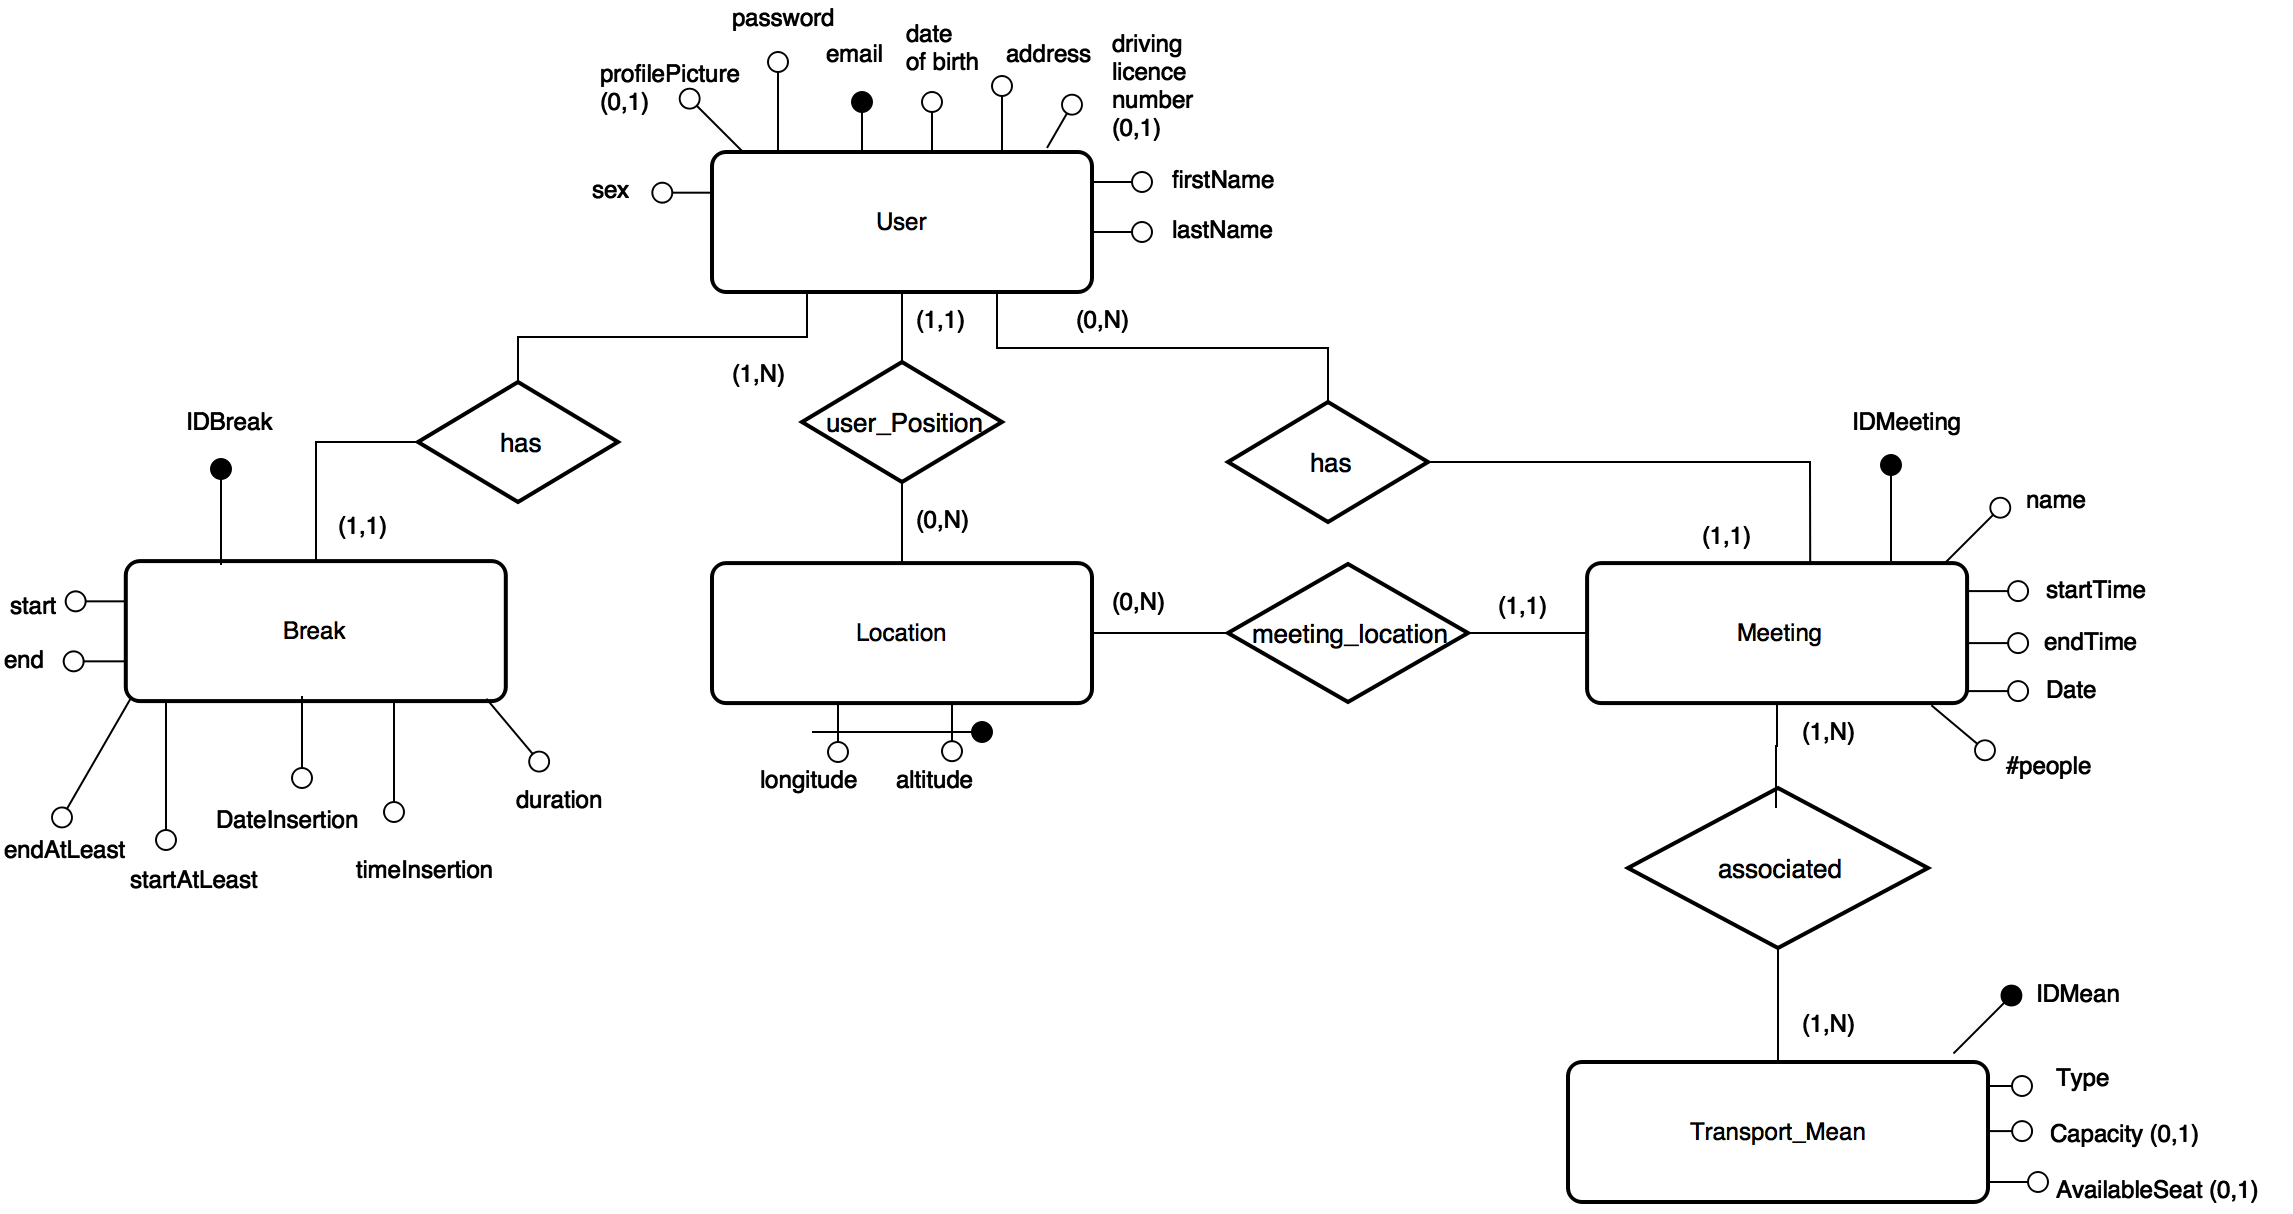
\includegraphics[width=\textwidth]{img/diagrams/er.png}
	\caption{ER Diagram.}
	\end{figure}


	\subsubsection{Application Server}
	This layer must handle business logic, data layer connections, and application access modes from different clients and external systems.
	
	The main feature of Application Server is the specific business logic modules that describe business rules and workflows for each feature provided by the application itself.
	
	The interface with the data layer must be managed by a dedicated persistence unit to ensure that only the Application Server can access the database.
	
	\bigskip
	Application Server must provide a means of interfacing with the Web Server and mobile clients through specific APIs in order to separate the different levels from their individual implementation. It must provide a way to communicate with external systems by adapting the application to existing external infrastructures.
	
	\bigskip
	The main business logic modules must include:

	\begin{description}
	\item [UserManager:] this module must manage all the logics concerning to user account creation, login and management.
	\item [EventManager:] this module must contain all the logic needed to create and modify meetings and breaks. It must guarantee the consistency of the model preventing from overlapping among events. 
	\item [MapManager:] this module must contain all the logic used to locate users and meetings. 
	\item [TravelInformationProvider:] this module must be able to interface with external agents such as \textit{Travel Information Providers} (i.e., ATM, Trenord, Alitalia, etc.).
	\item [NotificationManager:] this module must be able to notify the user when it is necessary to do so (e.g. an user tries to insert a meeting that overlaps with a previous one).
	\end{description}


	\subsubsection{Web Server}
	The Web Server Layer is responsible to provide the web pages to the users that intend to access the application's services via web.
	
	\bigskip
	This layer does not contain any application logic; it only provides static web pages that, through propers scripts (Javascript), are able to access the REST APIs of the Application Server and make it accessible to end users.

	\bigskip
	The scripts must be able to consume all the API's endpoints for the functionalities intended to be accessible via web.
	The communication with the APIs must be through textual data files over HTTPS (e.g. XML or JSON), as previously specified in \textit{Application Server} section.


	\subsubsection{Mobile Application Client}
	The Mobile Application Client must be designed to allow easy communication and implementation independent with the Application Server.
	The mobile application user interface should be designed following the guidelines provided by Android and iOS producers.
	The application must provide a software module that manages the GPS connection so that it can track location data by providing it to application servers.


	\subsubsection{Web Application Client}
	A \textit{Web Application Client} is any modern browser (eg., IE, Firefox, Chrome, Safari) able to run Javascript to allow the pages to consume the REST APIs of the \textit{Application Server}.


	\subsubsection{Implementation Choices}

	\textbf{Database Implementation}

	\medskip
	\noindent
	The \textit{Data Layer} must respect the following constraints: 
	\begin{itemize}
	\item Relational DBMS;
	\item MySQL 5.7 as DBMS implementation;
	\item JPA as database interface in the \textit{Application Server}.
	\end{itemize}

	\bigskip
	\noindent
	\textbf{Application Server Implementation}

	\medskip
	\noindent
	In this layer the central character is JEE7.
	This choice grants us several benefits such as security, reliability and availability.


	More specifically:

	\begin{itemize}
	\item GlassFish Server as \textit{Application Server} implementation;
	\item Enterprise JavaBeans (EJB)
	\item JavaPersistenceAPI (JPA)
	\item JAX-RS to implement proper RESTful APIs
	\end{itemize}

	\bigskip
	\begin{figure}[!ht]
	\centering
	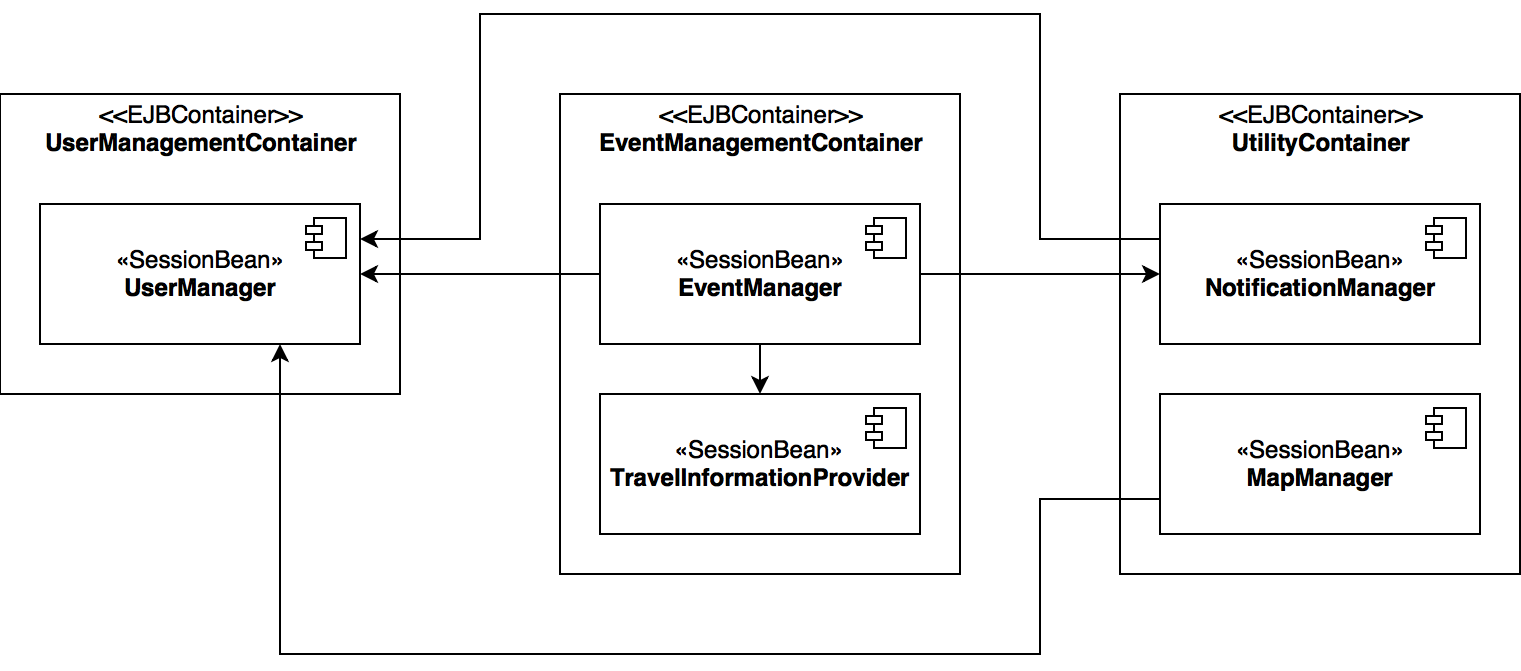
\includegraphics[width=\textwidth]{img/diagrams/asc.png}
	\caption{The components of the Application Server. An arrow going from component A to component B means that A uses interfacing methods provided by B.}
	\end{figure}

	\newpage
	\bigskip
	\noindent
	\textbf{Web Server Implementation}

	\medskip
	\noindent
	The main choice for this layer is to use NGINX 1.12 as web server.

	NGINX is the most widely used web server implementations, is event-driven and will grant us reliability and efficiency handling HTTP(S) requests.

	\bigskip
	The \textit{web server} will serve static files, i.e. html, css, javascript files, that will be interpreted client-side.

	Web pages must be able to connect to the \textit{application server}'s REST APIs and allow the user to access all the functionalities of the system through a web interface.


	\bigskip
	\noindent
	\textbf{Mobile Application Implementation}

	\medskip
	\noindent
	There must be two \textit{mobile application client} implementations to support both iOS and Android OSs:
	\begin{description}
		\item [iOS:] This implementation must be written in Swift using UIKit.
		\item [Android:] This implementation must be written in Java.
	\end{description}

	\bigskip
	\noindent
	Both of them must:
	\begin{itemize}
	\item Communicate with the \textit{application server} through the REST APIs over HTTPS.
	\item Follow the design guidelines provided by the devices' vendors.
	\end{itemize}

	\subsection{Deployment view}
	\begin{figure}[!ht]
	\centering
	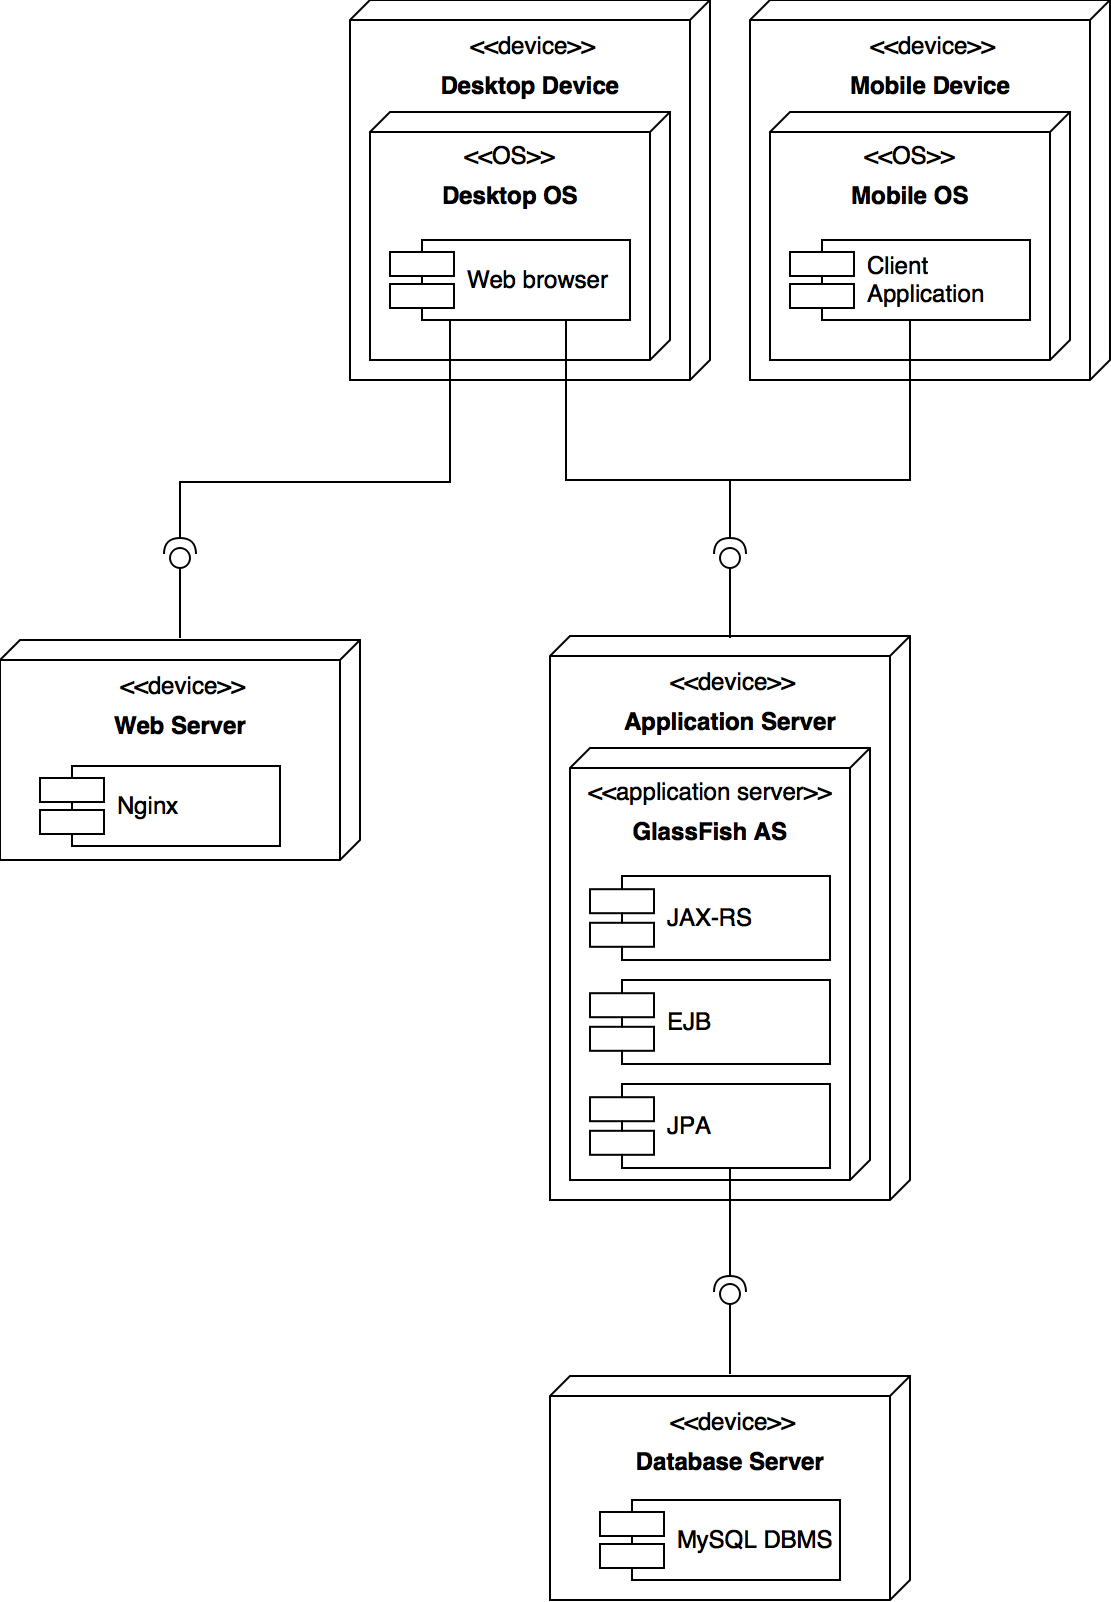
\includegraphics[width=0.75\textwidth]{img/diagrams/dv.png}
	\caption{Deployment View Diagram.}
	\end{figure}


	\newpage
	\subsection{Runtime view}
	This section describes the dynamic behavior of the system in the most relevant cases.

	The sequence diagrams, shown below, highlight the runtime interactions between client, server, and database.
	
	\bigskip
	Interactions are expanded and analyzed in detail when there are internal interactions between subcomponents of the Application Server.
	
	Direct interactions between Application Server and Database are not explicitly represented because they are abstract by the persistence unit of the Application Server.

	\bigskip
	\begin{figure}[!ht]
	\centering
	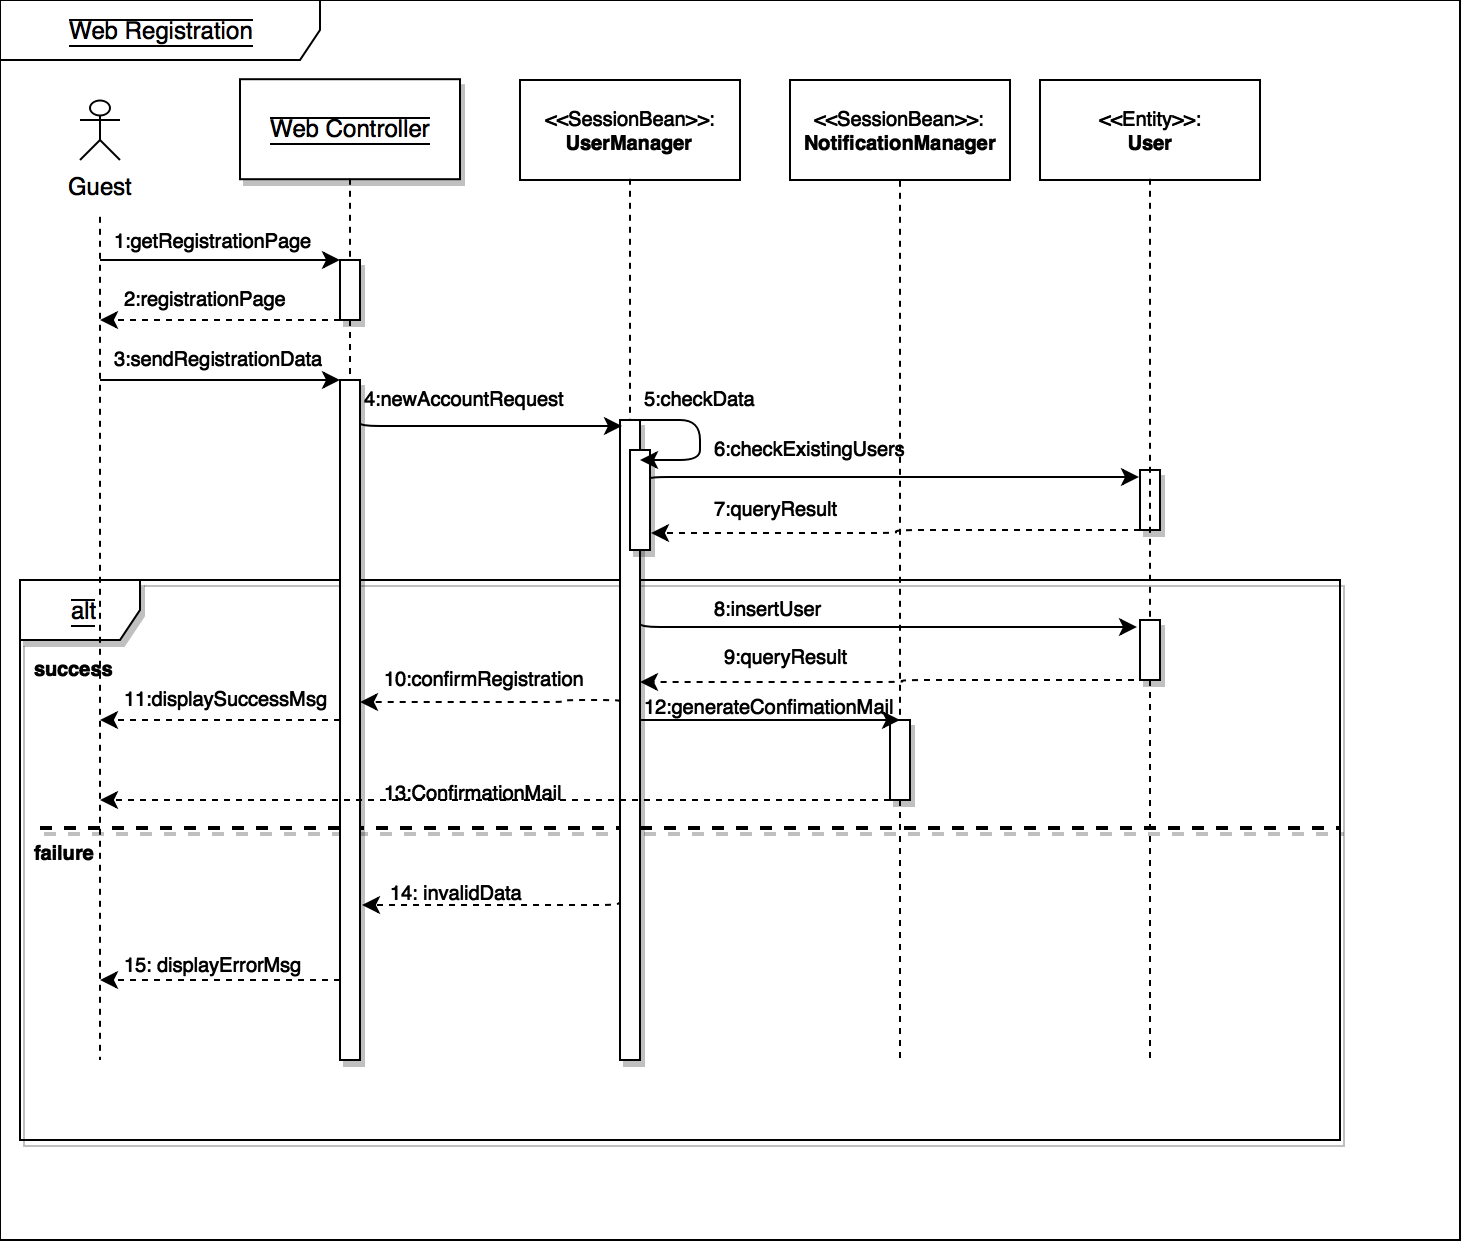
\includegraphics[width=0.8\textwidth]{img/diagrams/sd_registration.png}
	\caption{Registration \textit{sequence diagram}.}
	\end{figure}
	\clearpage

	\begin{figure}[!ht]
	\centering
	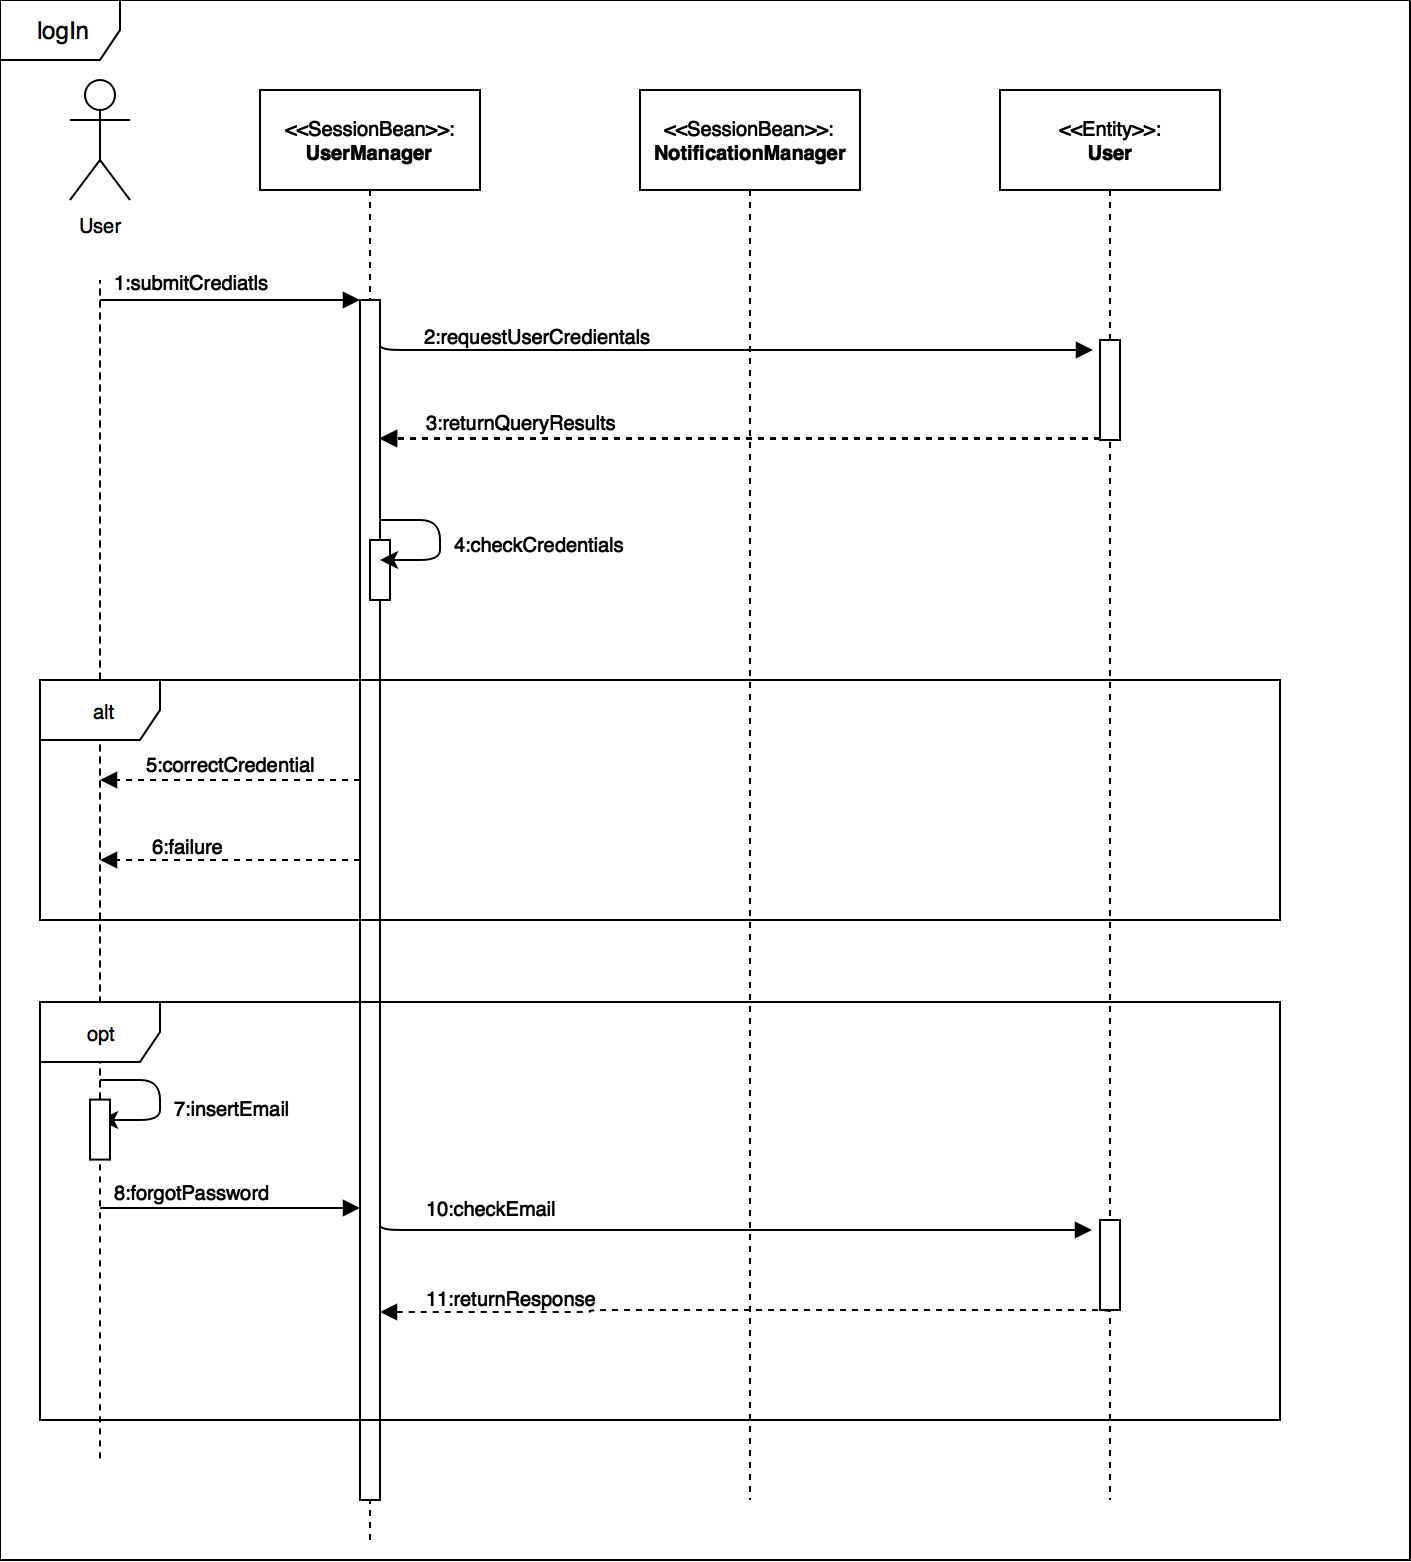
\includegraphics[width=0.8\textwidth]{img/diagrams/sd_login.png}
	\caption{Login/Credentials recovery \textit{sequence diagram}.}
	\end{figure}

	\begin{figure}[!ht]
	\centering
	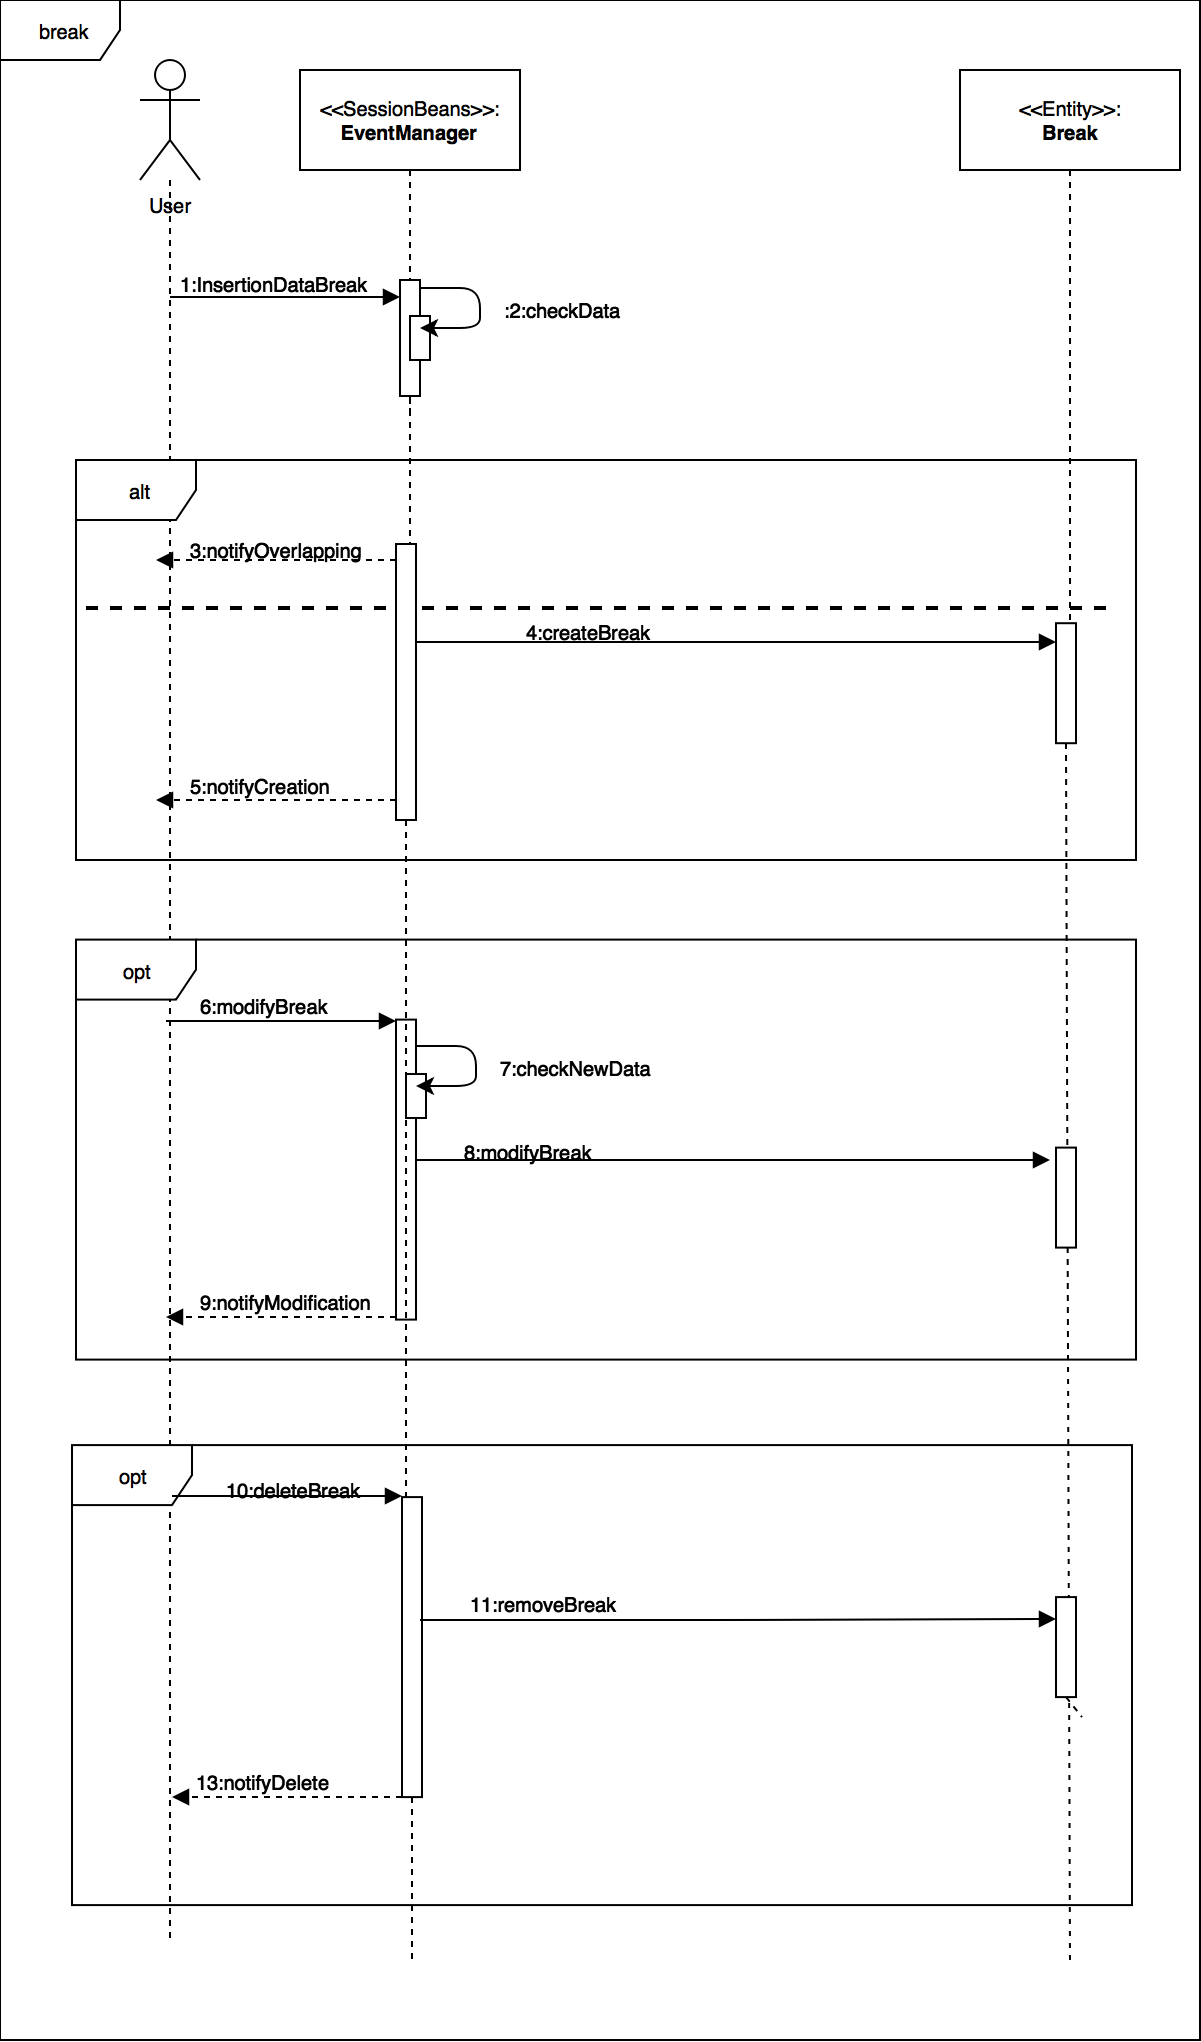
\includegraphics[width=0.8\textwidth]{img/diagrams/sd_meeting.png}
	\caption{Meeting creation, modification and deletion \textit{sequence diagram}.}
	\end{figure}

	\begin{figure}[!ht]
	\centering
	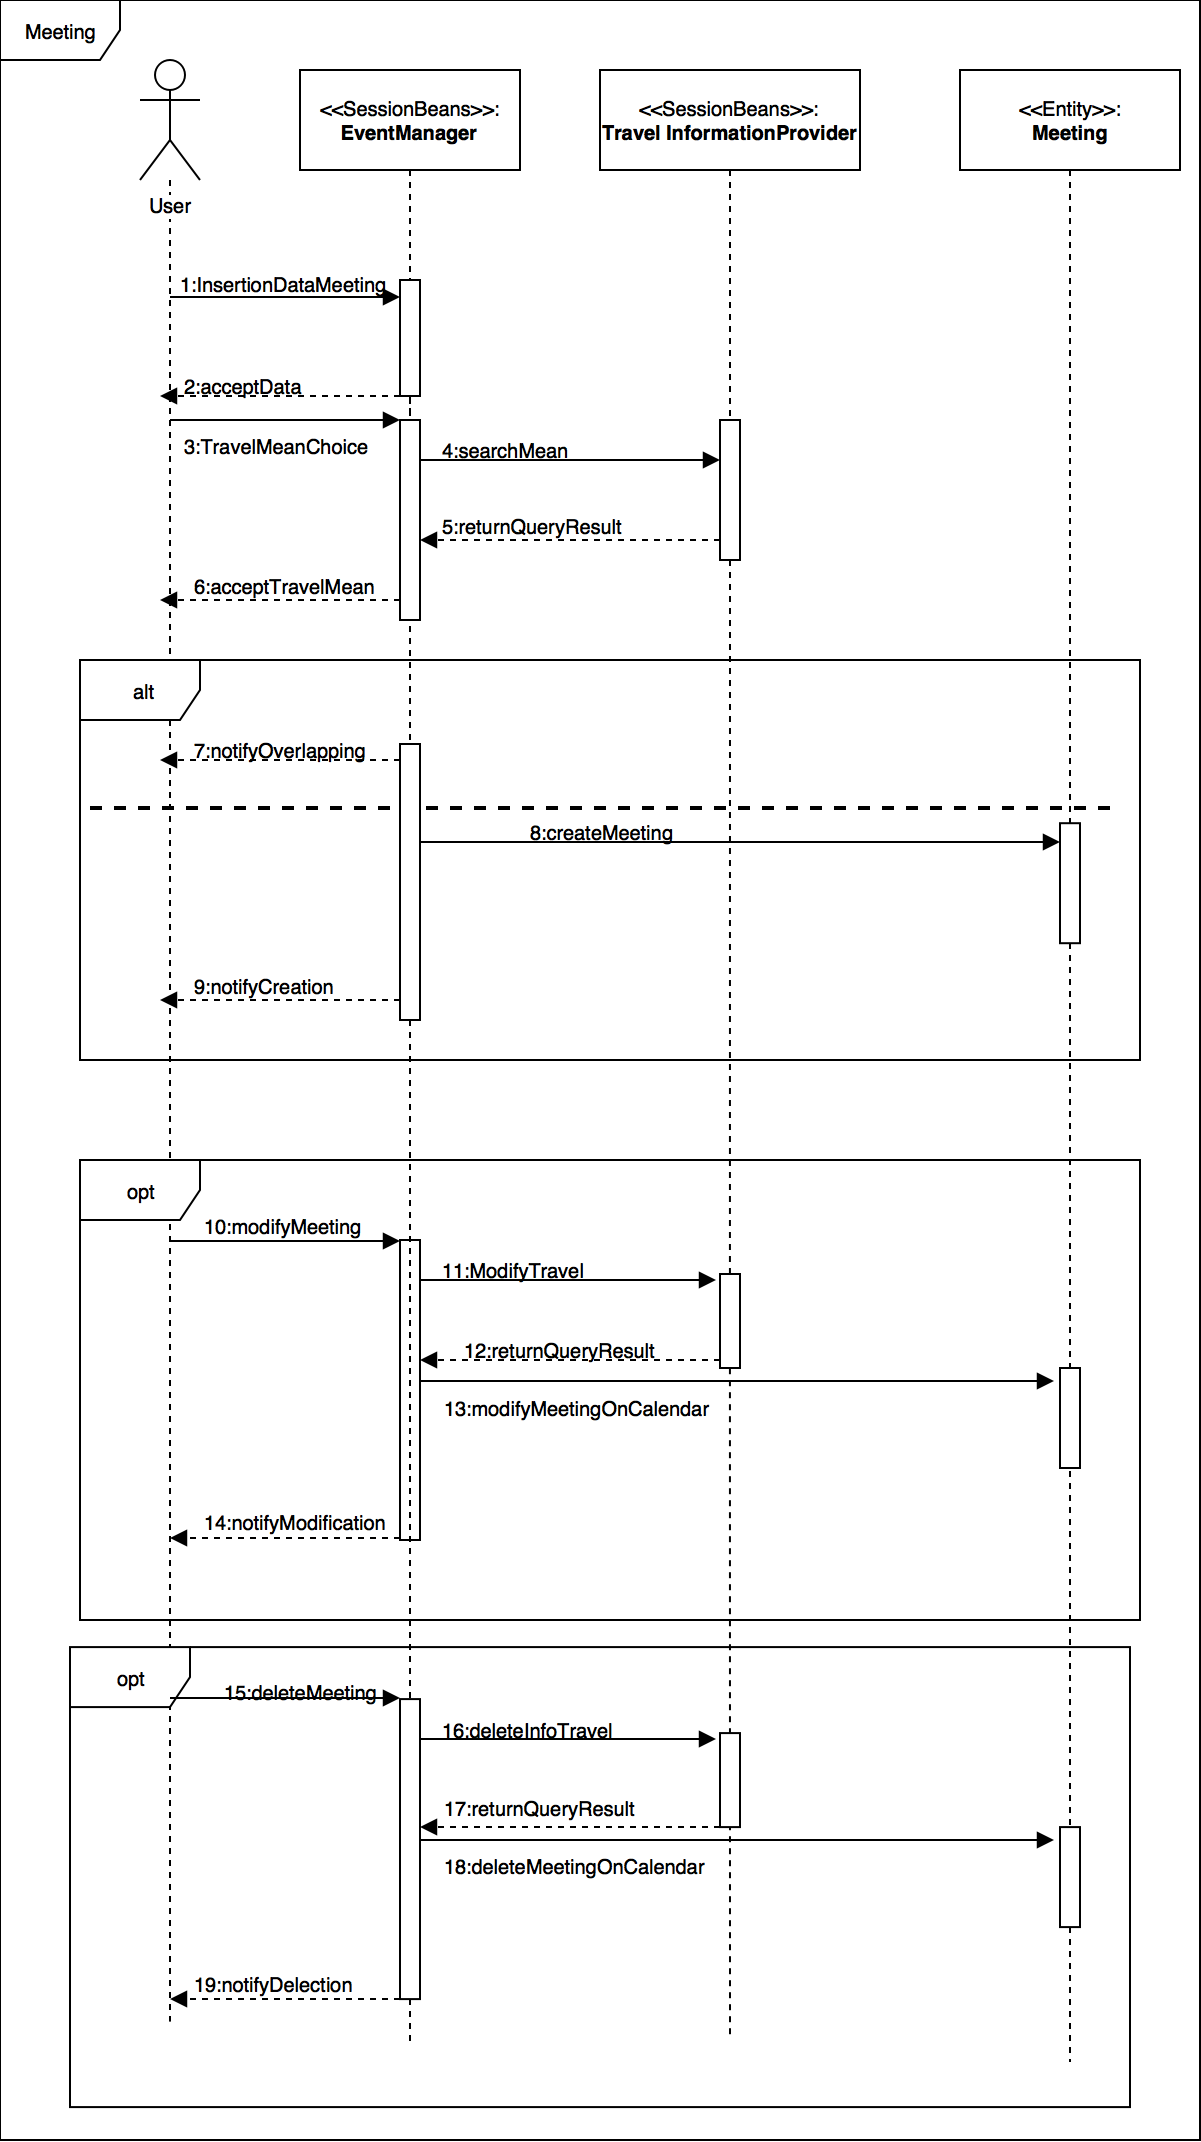
\includegraphics[width=0.75\textwidth]{img/diagrams/sd_break.png}
	\caption{Break creation, modification and deletion \textit{sequence diagram}.}
	\end{figure}


	\newpage
	\subsection{Component interfaces}
	
	This section of the Design Document describes in detail the interfaces of the various components of the system. The various sections underline the relevant details about the interfaces required to use and interact with each component of the Application Server.

	\subsubsection{Database - Application Server}
	The Application Server is the only one that can access the Database directly through the Java Persistence API mapping between objects and actual relations.


	\subsubsection{Web Server - Web Browser}
	As described in the RASD document [1], interactions between client’s  browsers and Web Servers are based on the HTTPS protocol.


	\subsubsection{Application Server - Web Server and Clients}
	The communication between the Application Server and the clients must take place via the RESTful APIs provided by the Application Server and implemented using JAX-RS.


	\subsubsection{Application Server - External Systems}
	Application Server must connect with the following external system:
	\begin{itemize}
	\item One or more travel and transport operators that use the interface APIs to which the Application Server must adapt in order to deal with or search for travel solutions.
	\end{itemize}


	\subsubsection{Internal interfaces for Application Server Components}
	\bigskip
	\noindent
	\textbf{UserManager}
	
	\bigskip
	\noindent
	The \textit{UserManager} interacts with the following entities:
	\begin{itemize}
	\item \textit{user} entity, in order to create, update, and delete user information during the registration process and check credentials during login to the application.
	\item \textit{location} entity, in order to always update user's position during any procedure.
	\end{itemize}

	\bigskip
	The procedures implemented by the \textit{UserManager} are:
	\begin{description}
	\item [submitLoginCredentials] -- This procedure is used to submit login credentials in order to access the application. The procedure takes the parameters as the email address and the password; if corrected, this function will have such a value for the user to perform other functions; if the credentials do not exist or are wrong, the return value is an error.
	\item [forgotPassword] -- this procedure is used when the user has forgotten the login credentials for the application. It returns a link to reset password.
	\item [registerUser] -- This procedure is used to request the creation of a new Travelendar + account; this takes as parameters all your personal information required for registration, in particular: first name, last name, sex, date of birth, address, email, password and driver's license number (optional); the return value for the procedure is an error when sending invalid data or a confirmation message in case of success.
	\item [deleteUser] -- This procedure is used to permanently delete a user account from the system; this does not require any parameter other than user authentication; the return value for this procedure is a confirmation message.
	\item [editProfile] -- This procedure is used whenever a user wishes to modify any information about his/her personal profile; this takes as a parameter a set of modified elements; the return value for this procedure is an error when entering invalid data, otherwise a confirmation message.
	\item [updateCurrentPosition] -- This procedure has the task of keeping the user's position updated. It takes the coordinates of the user’s place as parameters and sends it to the Map Manager to calculate the position; in case of failed sending returns an error message.
	\end{description}

	\bigskip
	\noindent
	\textbf{EventManager}

	\bigskip
	\noindent
	The \textit{EventManager} interacts with the following entities:
	\begin{itemize}
	\item \textit{meeting} entity, in order to create, edit and delete meetings in the calendar.
	\item \textit{location} entity, in order to set the location of a meeting.
	\item \textit{brake} entity, in order to create, edit and delete brakes in the calendar.
	\item \textit{transport\_mean} entity, in order to calculate how to reach a meeting.
	\end{itemize}

	\bigskip
	The procedures implemented by the \textit{EventManager} are:
	\begin{description}
	\item [createMeeting] -- This procedure is used to submit meeting information on meeting creation. The procedure takes as parameters \textit{name}, \textit{startTime}, \textit{endTime}, \textit{location}, \textit{peopleNumber}. On success the procedure returns the \textit{id} of the meeting.
	\item [editMeeting] -- This procedure is used to submit meeting information while editing a meeting. The procedure takes as parameters \textit{name}, \textit{startTime}, \textit{endTime}, \textit{location}, \textit{peopleNumber}. All the parameters are optionals and the procedure modifies only the ones that are not null.
	\item [deleteMeeting] -- This procedure is used to delete a meeting. The procedure take as parameter the meeting's \textit{id}.
	\item [getMeeting] -- This procedure is used to retrieve detailed information of a meeting. The procedure takes as parameter the \textit{id} of the meeting.
	\item [getMeetings] -- This procedure is used to retrieve a list of meetings according to the filtering fields. The procedure takes as parameters \textit{after} (default = now), \textit{before} (default = now + 7 days), \textit{near}, \textit{radius}, \textit{limit} (default = 15). All the parameters are optionals.
	\item [createBreak] -- This procedure is used to submit break information on break creation. The procedure takes as parameters \textit{name}, \textit{minStartTime}, \textit{maxEndTime}, \textit{duration}. On success the procedure returns the \textit{id} of the break
	\item [editBreak] -- This procedure is used to submit break information while editing a break. The procedure takes as parameters \textit{name}, \textit{minStartTime}, \textit{maxEndTime}, \textit{duration}. All of the parameters are optionals and the procedure modifies only the ones that are not null.
	\item [deleteBreak] -- This procedure is used to delete a break. The procedure take as parameter the \textit{id} of the break.
	\item [getBreak] -- This procedure is used to retrieve detailed information of a break. The procedure takes as parameter the \textit{id} of the break.
	\item [getBreaks] -- This procedure is used to retrieve a list of breaks according to the filtering fields. The procedure takes as parameters \textit{after} (default = now), \textit{before} (default = now + 7 days) and \textit{limit} (default = 15). All the parameters are optionals.
	
	\end{description}

	\bigskip
	\noindent
	\textbf{MapManager}

	\bigskip
	\noindent
	The \textit{MapManager} interacts with the following entities:
	\begin{itemize}
	\item \textit{location} entity, in order to keep user’s position updated and calculate the location of the meeting. It also calculates the path to reach the meeting.
	\end{itemize}

	\bigskip
	The procedures implemented by the \textit{MapManager} is:
	\begin{description}
	\item [computeLocation] -- This procedure is used to keep the user's position updated and the location of the meeting; it takes coordinates as parameters and sends it to the external system that will calculate the position.
	\end{description}

	\bigskip
	\noindent
	\textbf{TravelInformationProvider}

	\bigskip
	\noindent
	The \textit{TravelInformationProvider} interacts with the following entities:
	\begin{itemize}
	\item \textit{user} entity.
	\item \textit{location} entity.
	\item \textit{travel\_mean} entity.
	\end{itemize}

	\bigskip
	The procedures implemented by the \textit{TravelInformationProvider} is:
	\begin{description}
	\item [computeTravel] -- This procedure computes which are the most suitable travel means to reach a certain location. The procedure takes as parameters \textit{fromLocation}, \textit{toLocation}, \textit{userPreferencies}. returns a list of suitable travel means according to user's preferences.
	\end{description}

	\bigskip
	\noindent
	\textbf{NotificationManager}

	\bigskip
	\noindent
	The \textit{NotificationManager} doesn't interact with any entity

	\bigskip
	The procedures implemented by the \textit{NotificationManager} are:
	\begin{description}
	\item [sendEmail] -- The procedure is used during the application processes to generate an e-mail message; this takes as a parameter the information entered by the user and those processed by external systems; the returned value is not defined because the e-mail (confirmation or error) is immediately sent.
	\end{description}


	\subsection{Architectural styles and patterns}
	The following architectural styles and patterns have been used:
	
	\bigskip
	\noindent
	\textbf{Client and server}
	
	\bigskip
	\noindent
	The client-server architecture is used at different levels in the Travlendar + system design:
	\begin{itemize}
	\item The mobile application is client with respect to the Application Server that receives and processes requests.
	\item The user’s browser, which is a system client, communicates with the Web Server, which has the task of providing the requested web page.
	\item The Application Server assumes client  role when querying the database.
	\end{itemize}	

	\bigskip
	\noindent
	\textbf{Multi - tiered architecture}
	
	\bigskip
	\noindent
	The multi - tiered client - server architecture allows to physically separate presentation, application processing, and data management operations.
	Moreover, in case of a Web Server failure, the system is accessible from the mobile application, so the number of system levels will increase in the availability of the service.

	\bigskip
	\noindent
	\textbf{Thin client}

	\bigskip
	\noindent
	The thin client approach has been following during the design phase for  the interaction among the users machines and the system itself.
	System logic is implemented by Application Server, which has sufficient computing power and can manage concurrency issues in an efficient way.
	Mobile application and user browser does not contain a decision logic, but only the presentation function is performed.
	This architectural choice allows users to enjoy the service through devices with limited computing power and easy updating software.

	\bigskip
	\noindent
	\textbf{Model View Controller}

	\bigskip
	\noindent
	The web and mobile applications follow the Model - View - Controller software design pattern.
	It divides the application into three interconnected parts. This is done to separate internal representations of information from the ways information is presented to, and accepted from, the user.

	\bigskip
	\begin{figure}[!ht]
	\centering
	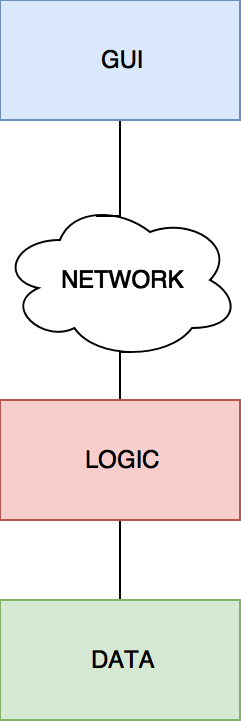
\includegraphics[width=0.15\textwidth]{img/diagrams/rp.png}
	\caption{The remote presentation architectural style that inspired the design of web/mobile application.}
	\end{figure}

	\newpage
	\subsection{Other design decisions}
	\subsubsection{User's passwords storage}
	Is good practice not to store user's passwords in plain text to prevent various kinds of cyberattacks. For this reason, this kind of sensible data must be ashed and salted before storing it in the database, preventing an attacker to know its actual value. 


	\subsubsection{Maps}
	As previously said, the application make use of maps to graphically show to the user the location of the events. For obvious reasons the system will make use of an external map service.

	The appointed service provider will be \textit{Google Maps}.


	\subsubsection{Travel Information Provider}
	To get informations about travel means schedules and routes we rely on an external services such as ATM APIs for the metropolitan area of Milan and Trenitalia for national travels, and so on and so forth.


	\section{Algorithm Design}

	\subsection{Most appropriate mean selection}
	As mentioned in the RASD document [1], the application are able to autonomously select the most appropriate travel mean to reach each meeting.

	This decision is the output of the following algorithm:
	\begin{enumerate}
	\item Ask the \textit{TravelInformationProvider} for a list of possible means to reach the meeting;
	\item Filter the list based on the user preferences (keep a mean only if the user selected it in his/her travel preferences);
	\item Check if the user wants to minimize his/her carbon footprint:
	\item \begin{enumerate}
		\item If yes, select the less polluting travel mean.
		\item If not, select the mean that takes the less time to reach the meeting.
		\end{enumerate}
	\item Done.
	\end{enumerate}


	\section{User Interface Design}


	\subsection{UX diagrams}
	The purpose of the UX diagram is to show the different screens provided by the user interface of an application and their dynamic content. It highlights the interactions between the different screens and the presence of input forms and data required on each screen.
 	
 	\bigskip
	The diagram shown below describes both the Web and Mobile applications, and follows the user interface requirements that are provided in the RASD document [1] (Figure 4.1).
 	
 	\bigskip
	The Web and mobile applications implement the same functionality.
 	
 	\bigskip
	It is emphasized that possible user choices are represented as input modules because they are data to be sent to the system and involve updating the screen.

	\begin{figure}[!ht]
	\centering
	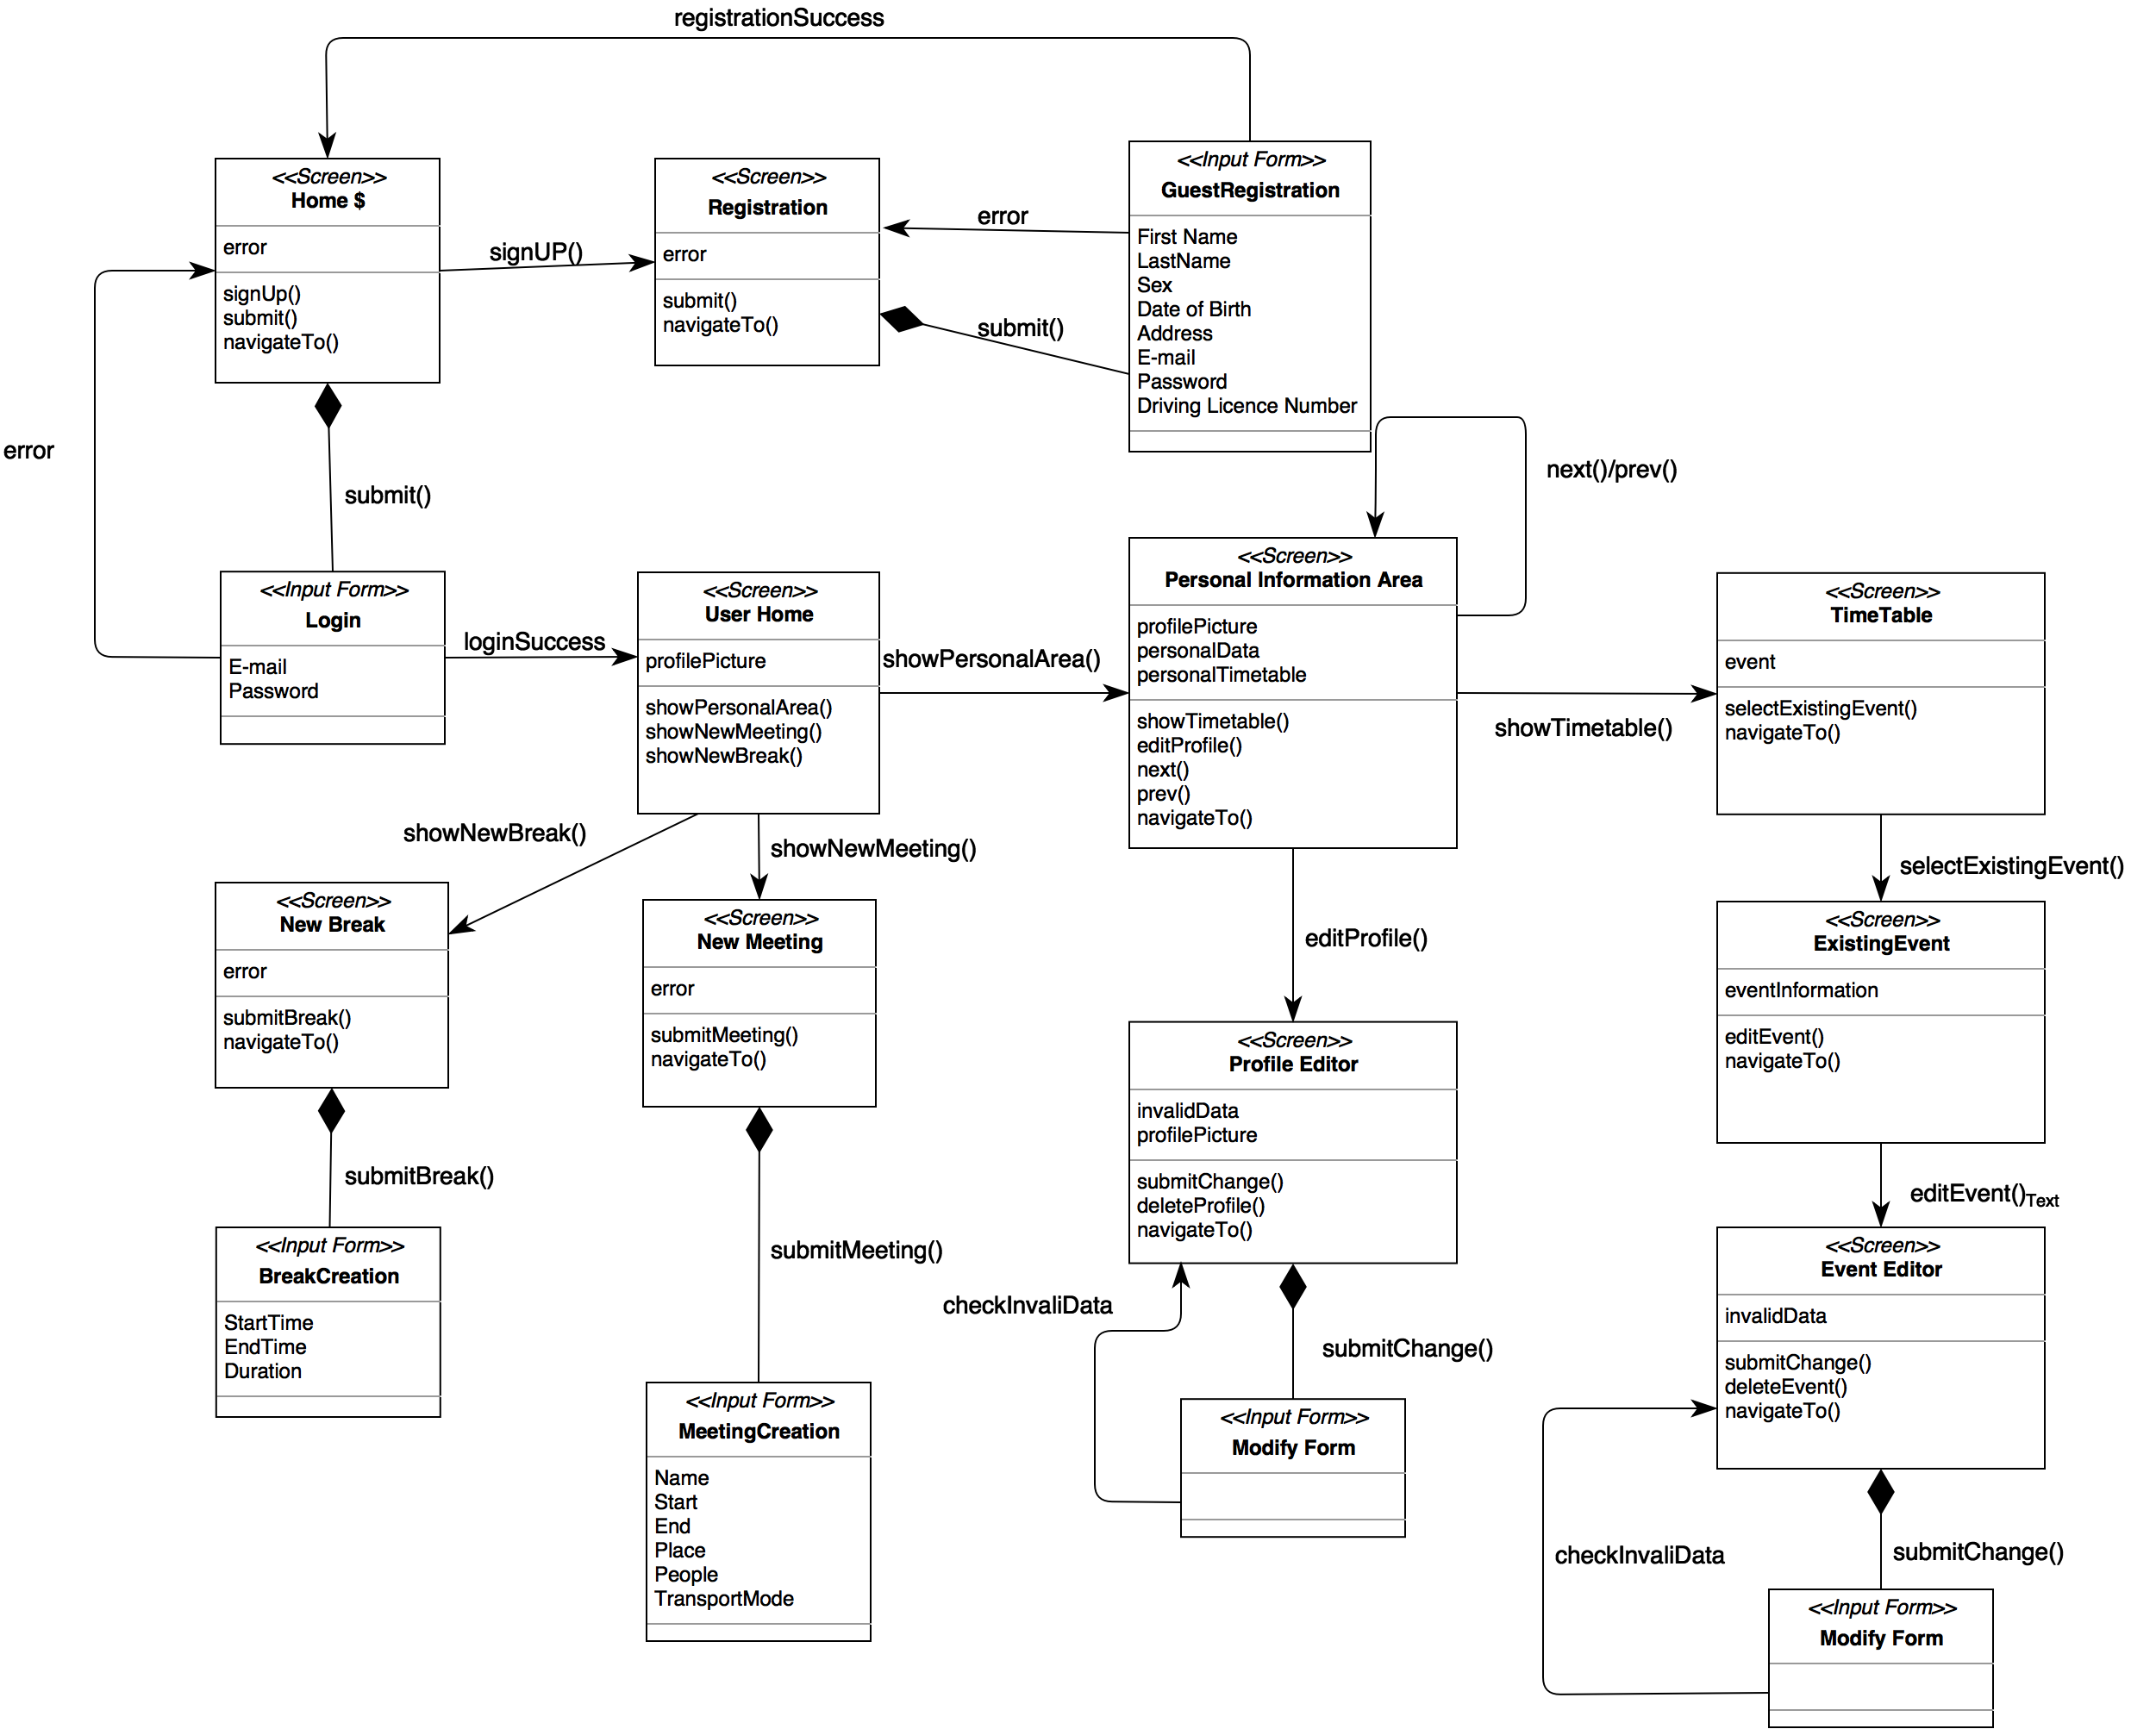
\includegraphics[width=\textwidth]{img/diagrams/ux.png}
	\caption{UX diagram of both Web and Mobile Application.}
	\end{figure}

	\subsection{User interface}
	\subsubsection{Web interface}
	The following mock-ups show how the interface of the Web Application should look like on the user’s browser.

	\subsubsection{Mobile interface}
	The following mock-ups show how the interface of the Mobile Application should look like on the user’s mobile devices.


	\subsubsection{Web interface}


	\subsubsection{Mobile interface}


	\section{Requirements Traceability}

	\subsection{Functional requirements}
	The following table (Table 5.1) is aimed to map the functional requirements described in the RASD document [1] to the components in the Design Document (only application logical components).

	\begin{center}
		\bigskip
		\begin{tabular}{|p{0.1\textwidth}|p{0.3\textwidth}|p{0.4\textwidth}|}
			\hline
			\textbf{Goal} & \textbf{DD Components} & \textbf{RASD Requirements} \\
			\hline
			1 \newline 2 \newline 3 & UserManager & 3.2.1 Register \newline 3.2.2 Login \newline 3.2.6 Manage profile information \newline 3.2.7 Delete profile \\
			\hline
			4 \newline 5 \newline 6 \newline 10 \newline 11 \newline 12 & EventManager & 3.2.3 Create Meeting \newline 3.2.4 Modify Meeting \newline 3.2.5 Delete Meeting \newline 3.2.10 Provide constraints \newline 3.2.11 Minimize Carbon Footprint \newline 3.2.12 Specify Break Timing \\
			\hline
			4 \newline 5 & Map Manager & 3.2.3 Create Meeting \newline 3.2.4 Modify Meeting \\
			\hline
			4 \newline 5 \newline 6 \newline 8 \newline 9 \newline 10 \newline 11 & TravelInformationProvider & 
			3.2.3 Create Meeting \newline 3.2.4 Modify Meeting \newline 3.2.5 Delete Meeting \newline 3.2.8 Activate Travel Mean(s) \newline 3.2.9 Deactivate Travel Mean(s) \newline 3.2.10 Provide constraints \newline 3.2.11 Minimize Carbon Footprint \\
			\hline
			1 \newline 1 \newline 4 \newline 5 \newline 10 \newline 12 & NotificationManager & 3.2.1 Register \newline 3.2.2 Login \newline 3.2.3 Create Meeting (overlap) \newline 3.2.4 Modify Meeting (overlap) \newline 3.2.10 Provide constraints \newline 3.2.12 Specify Break Timing \\ 
			\hline
		\end{tabular}
	\end{center}


	\subsection{Non-functional requirements}
	The following table (Table 5.2) illustrates the sections of the Design Document that highlight the subjects related to the satisfaction of the non-functional requirements in the RASD document [1].

	\begin{center}

		\bigskip
		\begin{tabular}{|p{0.4\textwidth}|p{0.4\textwidth}|}
			\hline
			\textbf{DD Section} & \textbf{RASD Requirements} \\
			\hline
			4 User Interface Design & 3.1.1 User Interfaces \\
			\hline
			2.6.2 Web Servers - Web Browsers & 3.1.4 Communications Interfaces \\
			\hline
			2.4 Deployment View & 3.4.1 Reliability \\
			\hline
			2.2 High level componets & 3.4.2 Availability \\
			\hline
			2.8 Other Decisions \newline 2.6.2 Web Servers - Web Browsers & 3.4.3 Security \\
			\hline
			2.3.6 Implementation Choices & 3.4.5 Portability \\
			\hline
		\end{tabular}
	\end{center}


	\section{Implementation, Integration and Test Plan}


	\subsection{Elements to be integrated}
	The integration test phase for the Travlendar + system will be structured according to the architectural division in the levels described in the first part of this document.
	
	The subsystems to integrate are as follows:
	\begin{description}
	\item [Database Tier] -- This includes all commercial database structures that will be used to store and manage system data, like the DBMS and the Database Engine; the component to be integrated is the DBMS.
	\item [Application Logic Tier] -- This includes all business logic for the application, data access components, and interface components to external systems and clients. All interactions must be tested and all subsystems that interact with this layer must be integrated individually.
	\item [Web Tier] -- This includes all components of the Web interface and communication with the application logic level and the browser client. Integration tests must be performed in both ways for this level.
	\item [Client Tier] -- Includes the Mobile application client, the Web browser client, and its internal components. Individual clients must behave correctly with respect to their internal structure and must be individually integrated with the level they interface with.
	\end{description}

	\subsection{Integration Testing Strategy}
	For the integration testing process, we decide to follow a bottom-up approach.
	
	This choice is natural since the integration testing can start from the smaller and the lowest level components, which have already been tested at the drive level, and do not depend on other components or not – already – developed components.
	
	The bottom - up strategy will be mixed with a critical-module-first approach to avoid major component failures and threats to the correct implementation of the entire Travlendar + system.
	
	The higher-level subsystems described in the previous paragraph are loosely coupled and sufficiently independent of each other because they correspond to different levels.
	
	To this purpose, the second cited approach is used to establish the correct integration order and to obtain the complete system.
	
	At this level of integration testing should also cover the communication functionalities with external systems.


	\newpage
	\appendix
	\section{Appendix}


	\subsection{Software and tools used}

	The software and tools used during the drawing of this document are:

	\begin{description}
	\item [LaTex:] used to build this document.
	\item [Google Drive / Google Documents:] used to always update and share the documents.
	\item [draw.io:] used to draw diagrams (https://www.draw.io).
	\item [Marvel:] used to build the mockups (https://marvelapp.com).
	\item [GitHub:] used as version control and to keep it shared between group members and teachers (https://www.github.com).
	\end{description}
	

	\subsection{Hours of work}

	Most of the work on this document was made in the presence of both members of the group. The approximate number of hours worked by each member of the group is as follow (including hours spent in group work):
	
	\bigskip
	Davide Rossetto: about 23 hours
	
	Alessandro Tatti: about 25 hours

	
	\section{Bibliography}
	
	\begin{description}
	\item [[1{]}] AA 2017/2018 Software Engineering 2 - Requirements Analysis and Specification Document - Davide Rossetto, Alessandro Tatti
	\item [[2{]}] AA 2017/2018 Software Engineering 2 - Project goal, schedule and rules
	\item [[3{]}] IEEE Standard 1016:2009 System design - Software design descriptions
	\end{description}

\end{document}
